\documentclass[11pt]{article}
\usepackage[left=1in, right=1in, top=1in, bottom=1in]{geometry}
\usepackage{titling}

\usepackage{graphicx}
\usepackage[export]{adjustbox}
\usepackage{caption}
\usepackage{subcaption}
\usepackage{hyperref}

\renewcommand{\arraystretch}{1.5}

\hypersetup{
    colorlinks=true,
    linkcolor=blue,
    filecolor=magenta,      
    urlcolor=cyan,
}

\graphicspath{ {images/} }

\setlength{\droptitle}{-5em} 
\pretitle{\begin{center}\Huge\bfseries}
\posttitle{\par\end{center}\vskip 0.5em}
\preauthor{\begin{center}\Large\ttfamily}
\postauthor{\end{center}}
\predate{}
\postdate{}

\title{Visualization Research Recommender \\ \large Visual Analytics project}
\author{Simone Bartolini 1752197}
\date{}
\begin{document}

\maketitle
\thispagestyle{empty}

\section{Introduction}
"What to do next?" This is the first question that comes to the mind of a researcher a soon as it has published a paper. He may continue to research the same topic as his latest publication or he may want to try to cover something different. This project proposes a visual analytics tool to help researchers explore the literature in the visualization field to find the best topics to study by analyzing their trends. In particular, the tool is based on the vispubdata dataset \cite{7583708}, which contains papers presented in one of SciVis, InfoVis, VAST or Vis conferences, from 1990 to 2020. 

The rest of this document is organized as follows:
\begin{itemize}
\item \autoref{sec:papers} is a review of papers that have addressed the same or similar problems and that have used similar techniques;
\item \autoref{sec:method} is a detailed description of the tool;
\item \autoref{sec:conclusions} contains my closing thoughts and some ideas on how the tool could be improved.
\end{itemize}



\section{Related papers} \label{sec:papers}
Over the years there has been a multitude of articles published with the aim of analyzing the structure and evolution of the scientific literature by extracting topics and studying their trends. When it comes to topic extraction, co-word analysis seems to be the more common approach, usually by clustering authors assigned keywords based on their co-occurrence using hierarchical clustering. \cite{Hu2013ACA} is an example of co-word analysis applied to the field of Library and Information Science (LIS), while \cite{7539364}, by the same authors of the vispubdata dataset \cite{7583708}, uses it to gather information about visualization publications, just like this project. Both show that keywords cannot be used directly but must first be preprocessed, to group different words referring to the same concept. They also noted the importance of filtering out higher-level keywords that are too broad. \cite{9373186} on the other hand demonstrates a more modern approach by using Machine Learning and Natural Language Processing to extract the topics from the full-text or the abstract of the articles. 

To visualize the results of the clustering, dimensionality reduction techniques like Multidimensional Scaling or T-Distributed Stochastic Neighbor Embedding are commonly used. Additionally, edges connecting keywords can be used to show their correlation forming a correlation network.

Finally to analyze the trends and find the most popular topics the two key parameters are the number of papers published covering a specific topic and the number of citations that those topics received. \cite{9079088} proposes an algorithm to extract the most trending topics, while \cite{9373186} illustrates a visualization tool that allows to interactively retrieving the information.

\section{Methodology} \label{sec:method}
\subsection{Dataset}
The selected dataset contains information on visualization publications from 1990 to 2020. Out of all attributes present in the dataset, these are the ones we are interested in:
\begin{itemize}
\item the conference where the paper was presented;
\item the year the paper appeared at the conference;
\item the title of the paper;
\item the digital object identifier (DOI);
\item the type of paper (conference paper, journal paper or miscellaneous);
\item the authors of the paper;
\item the references of the papers, i.e. the list of the DOIs of the cited papers;
\item and, most importantly, the keywords chosen by the authors.
\end{itemize}


\subsection{Topic extraction}
If the goal of the tool is to find the most promising topics, the first thing to do is define the topic list. The selected dataset contains a list of keywords for each article, but they are too specific (there are more than 5000 different keywords in a dataset of just over 3000 articles). Furthermore, different authors may have used different variations of a keyword to represent the same concept. Thus, to extract the topics, I decided to proceed in two phases:
\begin{enumerate}
\item \textbf{keywords deduplication: }I used a combination of automated clustering based on natural language processing and manual cleanup to group together the various keywords representing the same concepts. Examples of common variations are singular vs plural, capitalized vs lowercase, open vs closed vs hyphenated compound words or acronyms vs full phrases. This phase was carried as preprocessing of the dataset to produce the input data for the visualization.
 \item \textbf{keywords clustering into topics: }I then decided to use hierarchical clustering with Ward’s method to group the keywords based on their co-occurrence, as the more two keywords appear together the more likely they belong to the same topic, and I used the most common keyword in a cluster to name the topic. This phase is actually the first part of the interaction of the user with the tool: the user can control the clustering by adjusting the distance threshold, and additionally can filter out specific keywords. 
\end{enumerate}

 
 \subsection{The visualization tool}
User interaction with the visualization tool can be divided into two parts:
\begin{enumerate}
\item adjusting the clustering parameters to define the topics (figure \ref{fig:clustering});
\item analyzing the statistics of the topics to find the most promising ones (figure \ref{fig:trends}).
\end{enumerate}

 ~
 
To aid the user in the process of clustering the keywords, the tool shows:
\begin{itemize}
\item a table of all keywords with their occurrences: the user can deselect specific keywords by clicking on the respective rows, or can filter out keywords that are too common or too rare using a double range slider. This can be useful to filter out higher-level terms;
\item the number of keywords selected as input of the clustering and the resulting number of topics;
\item a table of the topics with the relative keywords, the number of papers covering the topic and their total citations count;
\item a scatter plot to help the user visualize the clustering results. It contains a point for each selected keyword, whose position is determined using TSNE (instead of MDS like in \cite{Hu2013ACA}, \cite{7539364} and \cite{9373186}) with as input the same co-occurrence matrix used for the clustering. Additionally, the point size is used to convey the frequency of the keyword. Finally, if the number of topics is not greater than 12, the points are color coded using the 'Paired' scheme, based on the topic they belong to. The colors assigned to the topics are also shown in the table of topics. Note that the limit of 12 is due to the fact that beyond this number it becomes difficult to distinguish colors quickly, in any case, passing over a point a tooltip will be displayed containing the name of the respective keyword and the related topic.
\end{itemize}

The user can select a topic to analyze from the relative table by clicking on it. This will populate the trend graph with the evolution over time of the number of published articles dealing with that topic and their citations, the list of papers will also be shown in a table. Note that the number of citations of a paper is computed based on the reference list of each paper so it only considers citations by other papers in the dataset. The user can also filter articles based on their type and the conference they appeared in. Additionally, it is possible to visualize the trends for a specific keyword or user-defined group of keywords by selecting them from the keywords' plot with a brushing action. 

 \begin{figure}[h!]
  \centering
  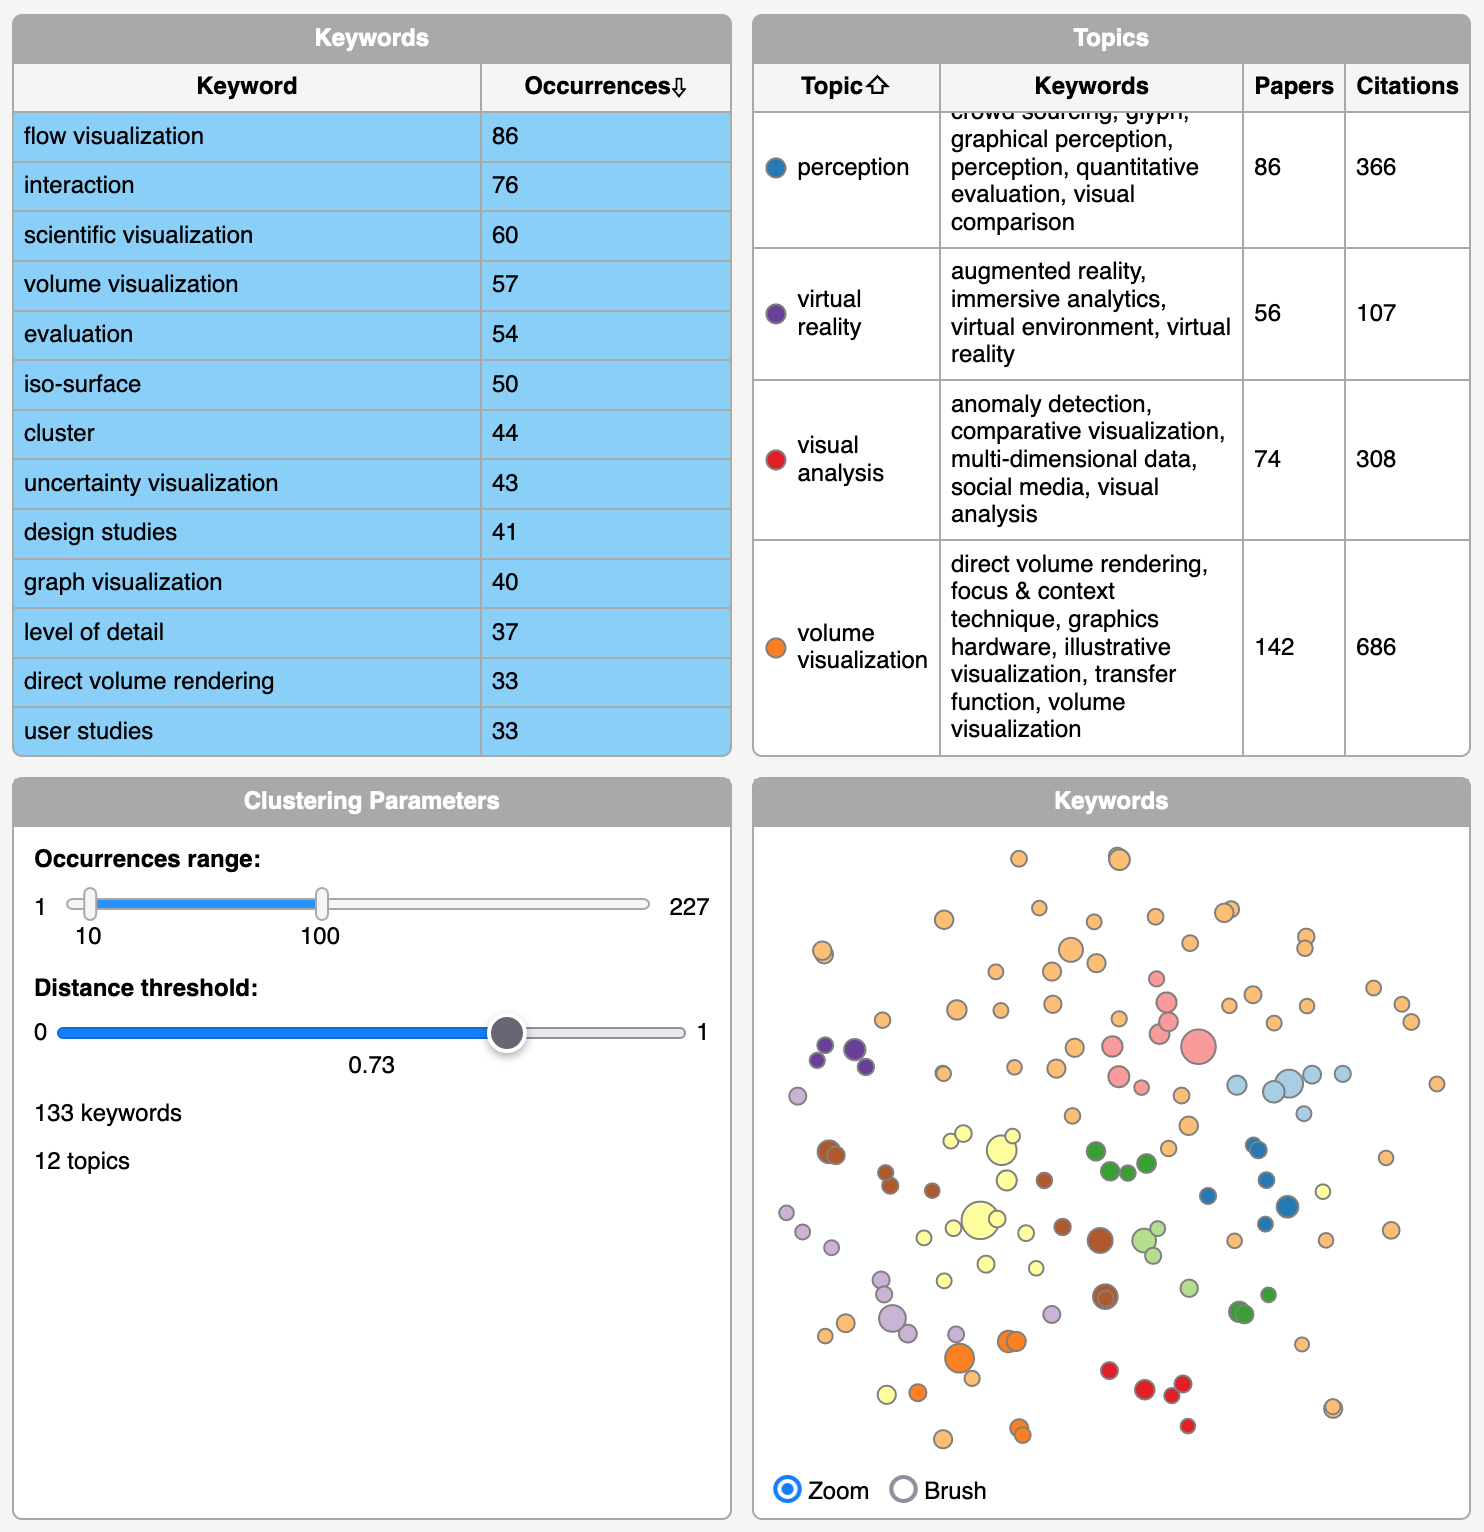
\includegraphics[width=0.6\linewidth]{clustering}
  \caption{Part of the visualization tool dedicated to clustering}
  \label{fig:clustering}
\end{figure}

 \begin{figure}[h!]
  \centering
  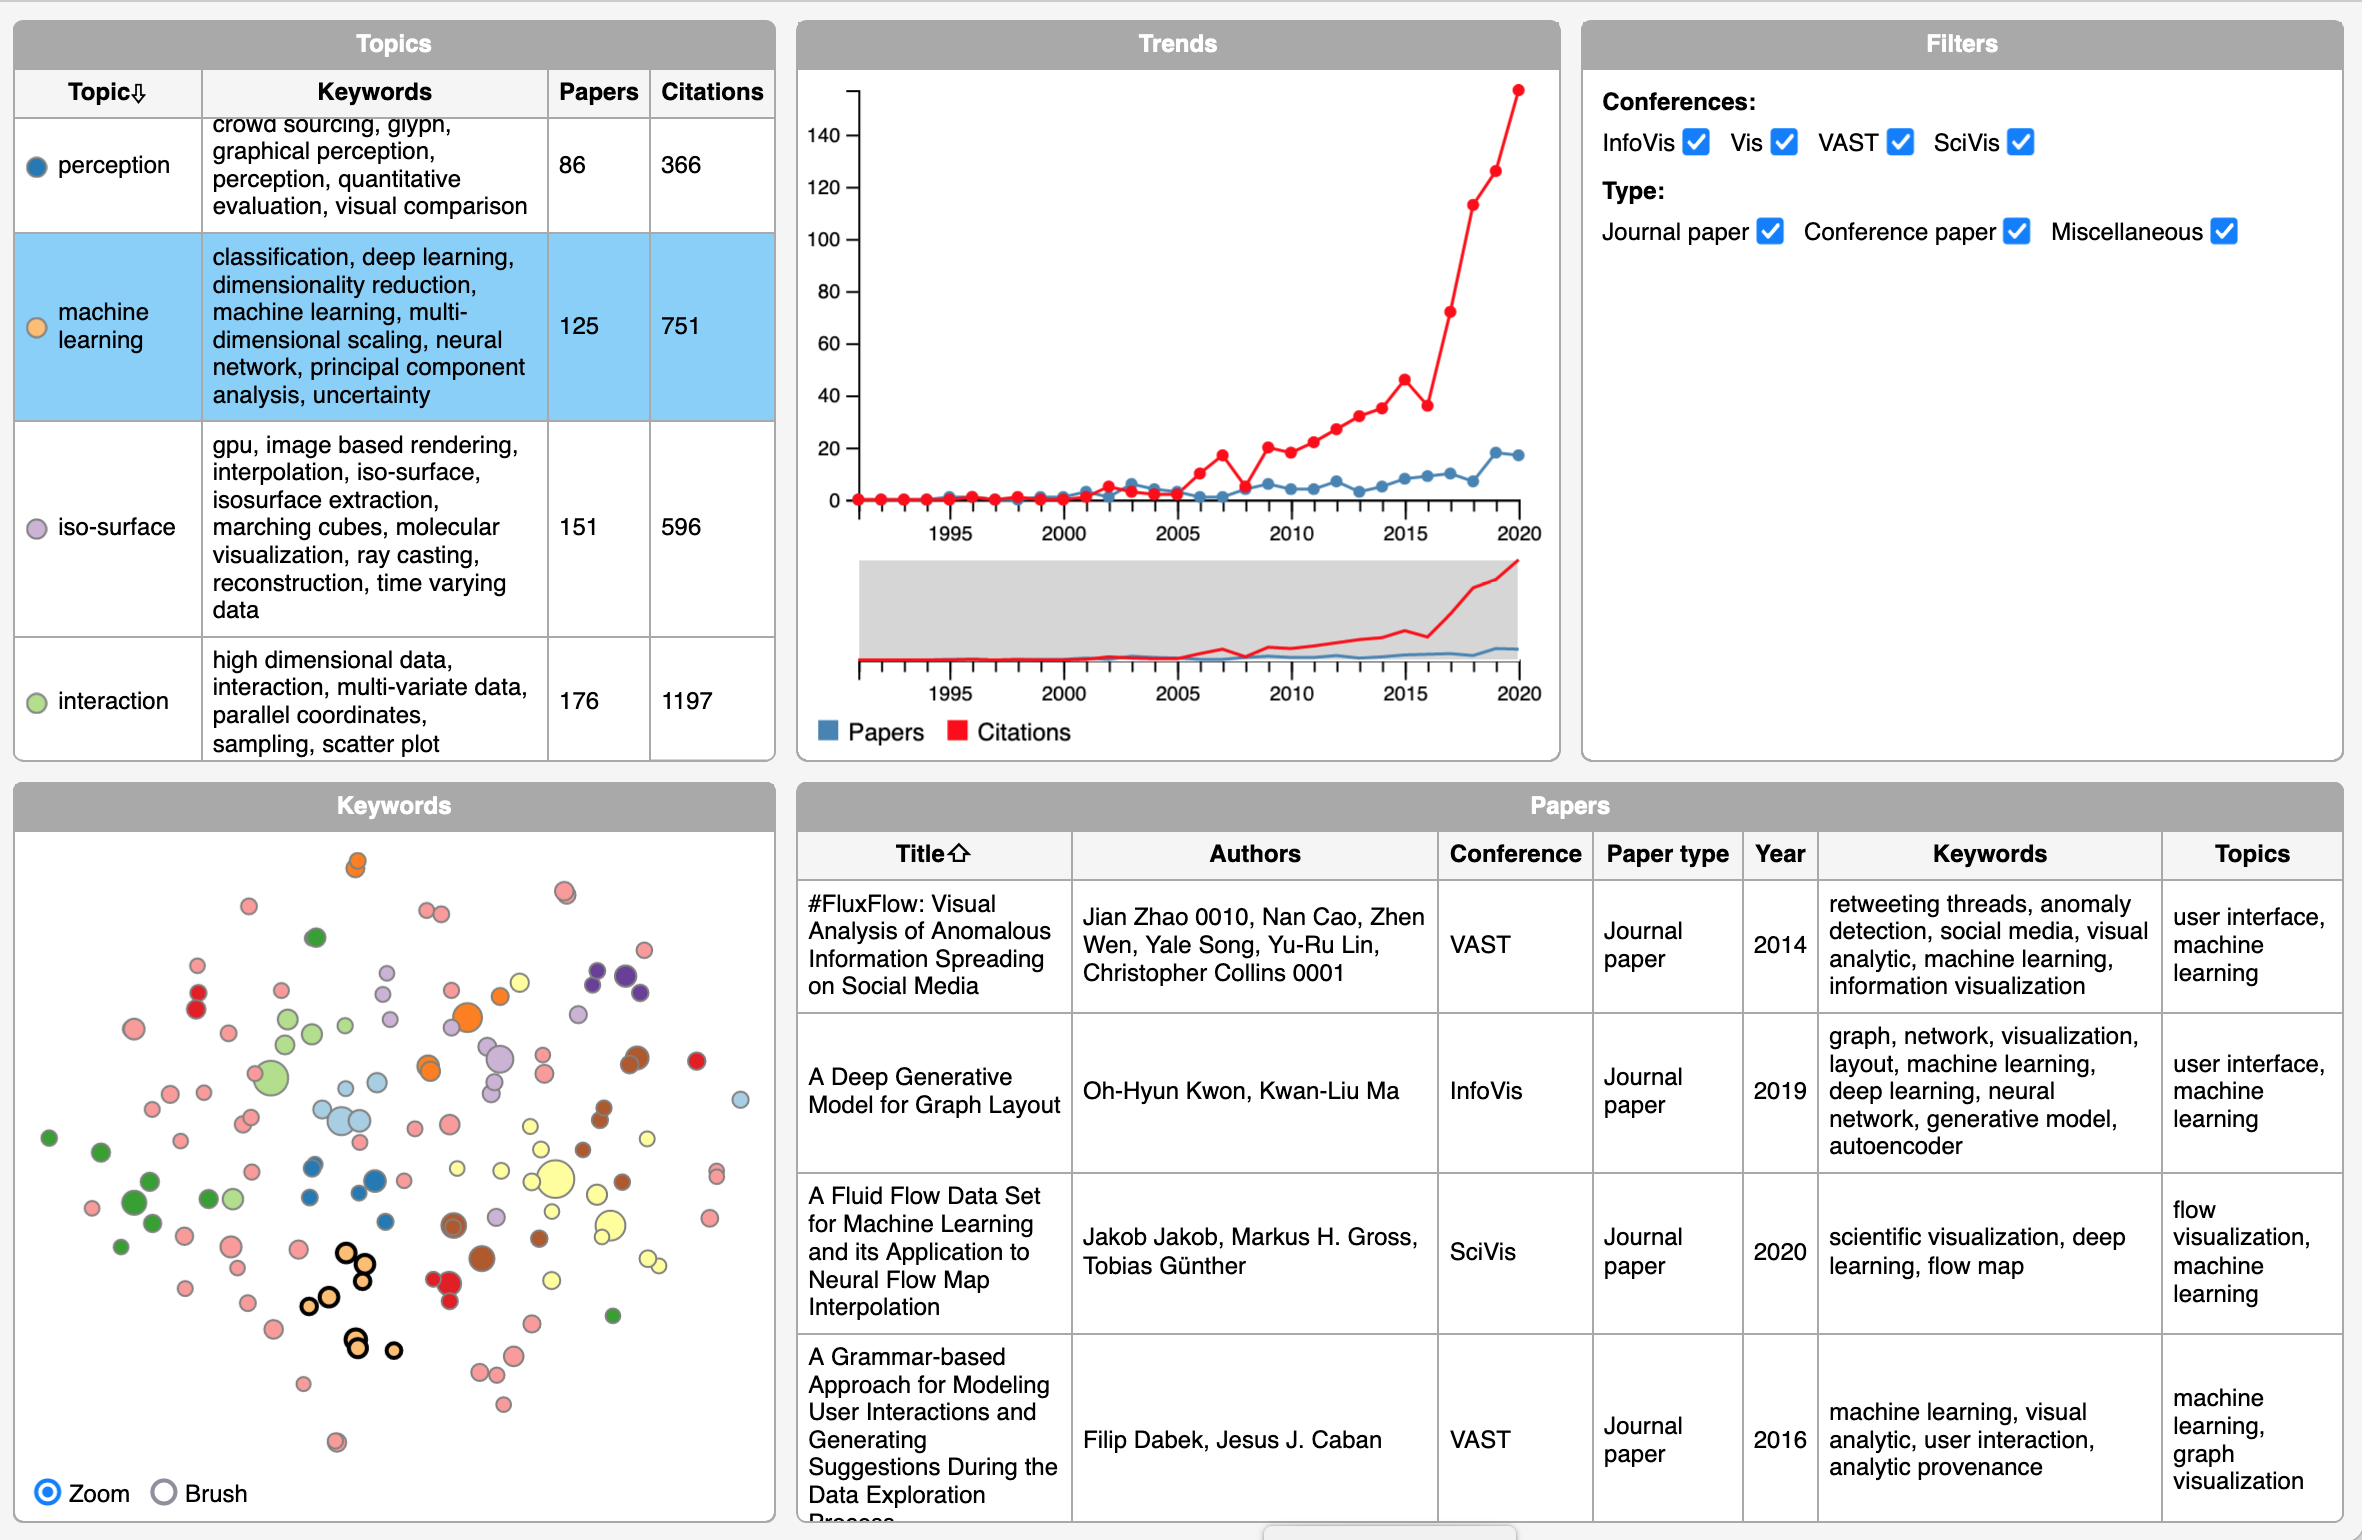
\includegraphics[width=0.9\linewidth]{trends}
  \caption{Part of the visualization tool dedicated to analyzing the evolution over time of the topics}
  \label{fig:trends}
\end{figure}

\newpage

\section{Conclusions and possible improvements} \label{sec:conclusions}
By carefully adjusting the parameters it is possible to extract representative topics and gather meaningful insights about them. For example, using the tool I was able to confirm that, unsurprisingly, the popularity of papers dealing with machine learning has grown dramatically over the past three to four years, and those papers generally get a lot of citations, while other topics, like volume rendering, they were very popular in the past, but are now on the decline.

However, the tool can certainly be improved. Other filters could be added to better explore the dataset, for example, it could be useful to be able to filter the papers based on the h-index of the authors or based on the reputation of their affiliation (additional data would though be needed to implement those). Furthermore, the visualization of the filters could be improved to give hints to the users regarding the distribution of the dataset. For example, a box plot of the keyword occurrence distribution could be shown under the occurrences range filter. Additionally, the plot of the keywords could be improved by adding edges that represent the correlation between keywords (like \cite{Hu2013ACA} and \cite{7539364} do) and by finding a way to be able to convey that a keyword belongs to a topic in a preattentive way even when the topics are more than 12. Also, right now the tool struggles with clustering keywords like 'focus+context' and 'focus+context technique' which share some words and are used interchangeably by authors to refer to the same concept. This could be solved by improving the preprocessing or by adding another clustering step in the tool at the beginning, based on string similarity (Note that \cite{7539364} used the brute force approach of manually reviewing the list of keywords to avoid this problem). Finally, a way to show the plot of the trends for more topics at a time would make comparing them much easier.

\newpage

\bibliographystyle{sapthesis}
\bibliography{bib} 

\end{document}